\documentclass[11pt]{arxiv}

\usepackage{minted}

\newcommand\fullsize{.92\textwidth}
\begin{document}

\title{How to Use arxiv Class}


\author{%
  \begin{tabular}{*{3}{c}}
  Saber \authormark[1] \authormark[2] & Lancer\authormark[2]& Rider\authormark[1]  \tabularnewline
  \email{saber@fate.org} & \email{lancer@fate.org} & \email{rider@fate.org} \tabularnewline
  Archer\authormark[2] & Gilgamesh\authormark[1] & Berserker\authormark[2]\tabularnewline
  \email{caster@fate.org} & \email{gilgamesh@fate.org} & \email{berserker@fate.org}\tabularnewline
  \authormark[1] Fate/Zero && \authormark[2] Fate/Stay Night \tabularnewline
  \end{tabular}      
}
\maketitle

\begin{abstract}
This article gives you a clear view of how to use the arxiv class to provide high quality
\textsc{LaTeX} submission for arXiv.
arxiv is a simple extension of {\code article.cls}.
This document is an example provided using arxiv class.

\end{abstract}


\section{Introduction}\label{sec:introduction}

The motivation of creating this \textsc{LaTeX} class is to make life simpler when dealing with arXiv submissions.


\section{Class Options}\label{sec:classOptions}

All options work for {\code article.cls} also work for this class.
For example,

\begin{minted}{TeX}
\documentclass[onecolumn]{arxiv}
\end{minted}


\section{``Clever'' Cross Reference}\label{sec:autoref}

This class provides {\code autoref} for referencing following LaTeX entities shown in~\autoref{tab: autoref}.

    \begin{table}[!htbp]
    \begin{center}\caption{Entities that have ``clever'' cross reference.}\label{tab: autoref}
    \begin{tabular}{@{}lll@{}}
    \toprule
    Entity & \textsc{LaTeX} Command & Result \\ \midrule
    Figure & \mintinline{latex}{\autoref{fig: custom-author-layout}} & \autoref{fig: custom-author-layout}\\ 
    Subfigure & \mintinline{latex}{\autoref{subfig: author-customization-one}} & \autoref{subfig: author-customization-one}\\
    Table & \mintinline{latex}{\autoref{tab: autoref}} & \autoref{tab: autoref}\\
    Equation & \mintinline{latex}{\autoref{eq: myeq}} & \autoref{eq: stationary-dist}\\
    Theorem & \mintinline{latex}{\autoref{thm: positive-recurrent}} & \autoref{thm: positive-recurrent}\\
    Proposition/Lemma/Corollary & \mintinline{latex}{\autoref{coro: compact}} & \autoref{coro: compact}\\
    Definition/Claim/Assumption & \mintinline{latex}{\autoref{def: borel}} & \autoref{def: borel}\\
    Section & \mintinline{latex}{\autoref{sec:introduction}} & \autoref{sec:introduction}\\
    Section in Appendix & \mintinline{latex}{\autoref{appsec: others}} & \autoref{appsec: others}\\
    \bottomrule
    \end{tabular}
    \end{center}
    \end{table}

\section{Theorem-like Environments}\label{sec: theorem-environment}

This class defines the following theorem-like environments: 
\begin{itemize}
\item Theorem: \mintinline{latex}{\begin{theorem}...\end{theorem}}
\item Corollary: \mintinline{latex}{\begin{corollary}...\end{corollary}}
\item Lemma: \mintinline{latex}{\begin{lemma}...\end{lemma}}
\item Proposition: \mintinline{latex}{\begin{proposition}...\end{proposition}}
\end{itemize}
All of them share the same counter, but as shown in~\autoref{sec:autoref}, they have different {\code autorefname}. 
Besides, we also provide the following ones, whereas each of them has its own counter.
\begin{itemize}
\item Definition: \mintinline{latex}{\begin{definition}...\end{definition}}
\item Claim: \mintinline{latex}{\begin{claim}...\end{claim}}
\item Assumption: \mintinline{latex}{\begin{Assumption}...\end{Assumption}}
\item Fact: \mintinline{latex}{\begin{fact}...\end{fact}}
\end{itemize}

\subsection{Some Examples}\label{subsec: theorem-like-env-examples}

\begin{proposition}\label{proposition: not-all-transient}
If $S$ is finite, then not all states can be transient. 
\end{proposition}

\begin{theorem}\label{thm: positive-recurrent}
Suppose that Markov chain is irreducible and aperiodic and that a stationary distribution $\pi$ exists with
\begin{equation}\label{eq: stationary-dist}
\pi^T = \pi^T P,
\end{equation}
and
\begin{equation}\label{eq: sum-to-1}
\sum_{j \in S}\pi_j = 1,\qquad \pi_j \ge 0.
\end{equation}
Then the Markov chain is {\bf positive recurrent}.
\end{theorem}

\begin{corollary}\label{coro: compact}
If $K_1, K_2,\cdots,K_N\in\mathbb{R}^n$ are compact, disjoint sets, then 
$$
\mid \bigcup_{j=1}^{N}K_j \mid_{e} = \sum_{j=1}^N\mid K_j\mid_e
$$
\end{corollary}

\begin{definition}[Borel $\sigma$-algebra]\label{def: borel}
The Borel $\sigma$-algebra in $\mathbb{R}^d$ is the smallest $\sigma$-algebra that contains all open sets in $\mathbb{R}^d$.
\end{definition}

\section{Packages Included \& Marcos Defined}\label{sec: packages-and-macros}

\subsection{Packages Included}\label{subsec: packages}

This class has included the following packages: {\code ifthen, latexsym, amsmath, amssymb, amsthm, graphicx, subfig, xcolor, 
cite, fullpage, verbatim, multirow, booktabs, url, etoolbox, appendix, aliascnt}. 

\subsection{Macros Defined}\label{subsec: macros}

This class defined the following macros: \mintinline{latex}{\code} (similar to \mintinline{latex}{\it}), 
\mintinline{latex}{\email} ({\it e.g.,} \mintinline{latex}{\email{saber@gmail.com}}), \mintinline{latex}{\authormark} (alias of \mintinline{latex}{\footnotemark}). 



% \newpage
\appendix

\section{Others}\label{appsec: others}

In the section, we will introduce some tricks that are applicable to \textsc{LaTeX} classes not limited to {\code arxiv}. 

\subsection{Customize Author Layout}\label{appsubsec: custom-author}
\begin{minted}{latex}
\author{%
  \begin{tabular}{*{6}{c}}
  Saber & Lancer & Rider & Caster & Gilgamesh & Berserker \tabularnewline
  \email{saber@fate.org} & \email{lancer@fate.org} & \email{rider@fate.org} 
  & \email{caster@fate.org} & \email{gilgamesh@fate.org} & 
  \email{berserker@fate.org}\tabularnewline
  \multicolumn{6}{c}{Fate Series Heroes}\tabularnewline
  \end{tabular}      
}
\end{minted}
The above code will give a result shown in~\autoref{subfig: author-customization-one}.
\begin{figure}[!htb]
\begin{center}
\subfloat[Example One.\label{subfig: author-customization-one}]{%
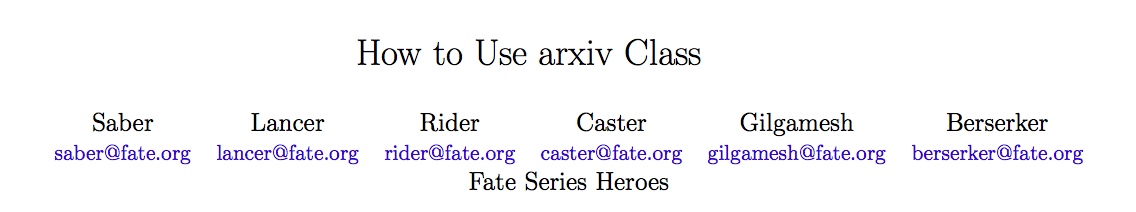
\includegraphics[width=\fullsize]{Figures/customized-authors-1}}\\
\subfloat[Example Two.\label{subfig: author-customization-two}]{%
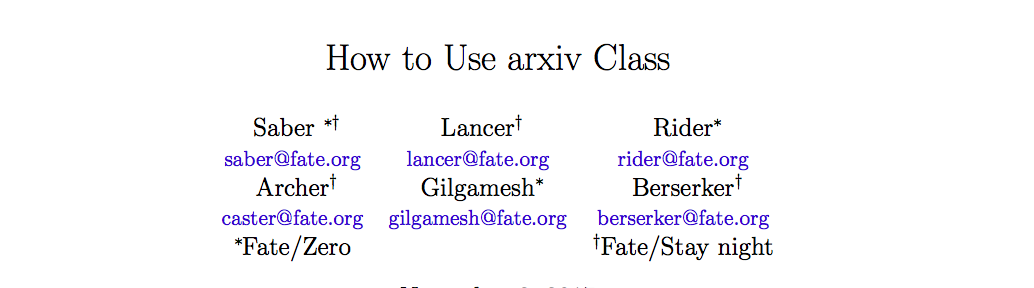
\includegraphics[width=\fullsize]{Figures/customized-authors-2}}
\end{center}
\caption{Customized author layout.}\label{fig: custom-author-layout}
\end{figure}
\begin{minted}{latex}
\author{%
  \begin{tabular}{*{3}{c}}
  Saber \authormark[1] \authormark[2] & Lancer\authormark[2]& 
  Rider\authormark[1]  \tabularnewline
  \email{saber@fate.org} & \email{lancer@fate.org} & 
  \email{rider@fate.org} \tabularnewline
  Archer\authormark[2] & Gilgamesh\authormark[1] & 
  Berserker\authormark[2]\tabularnewline
  \email{caster@fate.org} & \email{gilgamesh@fate.org} & 
  \email{berserker@fate.org}\tabularnewline
  \authormark[1] Fate/Zero && \authormark[2] Fate/Stay Night \tabularnewline
  \end{tabular}      
}
\end{minted}
The above code will give a result shown in~\autoref{subfig: author-customization-two}.
\end{document}